\chapter{基于蒙特卡罗采样的显著性区域检测}

\section{引言}
\subsection{研究背景}
对视觉显著性的研究最早可以追溯到Koch和Ullman的基于生物视觉原理的模型\cite{koch1987shifts},之后Itti等人融入了多尺度图像特征进行了改进\cite{itti1998model}。自此之后,显著性检测就吸引了来自各个领域的众多学者。

在最初的阶段,人们试图根据局部对比度挖掘图像区块的稀有性,从而去定义显著值。在Ma和Zhang的工作中\cite{ma2003contrast},首次结合了fuzzy growing与局部对比度分析用于显著区域检测。在Harel等人的工作中\cite{harel2006graph},根据相邻像素点的相似性首先构建了一个邻接图,然后利用马尔科夫过程来挖掘像素的显著性。其他学者,比如Liu等人\cite{liu2011learning},以及Mai等人\cite{maisaliency},都将局部对比度作为一个很重要的特征。

然而,基于局部对比度的方法倾向于给予边缘更高的显著值,而并非高亮整个显著区域。故近年来,越来越多的学者开始使用全局对比度。Zhai等人\cite{zhai2006visual}提出了第一个基于全局对比度的显著区域检测模型,然而,考虑到直接在三通道色彩空间上计算,时间复杂度太高,他们只采用了亮度信息进行计算。Cheng等人\cite{cheng2011global}则改进了这个算法,他们应用了三通道进行计算,为了减少时间复杂度,同时引入了量化和色彩空间平滑两个工具。

随着机器学习方法的火热,机器学习也被许多学者尝试应用于该领域。Kienzel等人\cite{zhai2006visual}基于眼动数据学习了一个kernel SVM,用于区分一个图像块是否显著。Ye等人\cite{ye2014salient}则采用了条件随机场,将局部和全局特征相结合,以弥补各个特征的缺陷。

\subsection{研究动机}
当前国际上的主流方法均有各自的缺陷:基于局部对比度的方法倾向于高亮边缘,而基于全局对比度的方法无法区分前景和背景中相同颜色的像素,基于学习的方法则与学习数据关系很大,在不同数据集上表现差异较大。同时,现有的方法时间复杂度都较高,实际利用价值大打折扣。

\begin{figure}
\centering
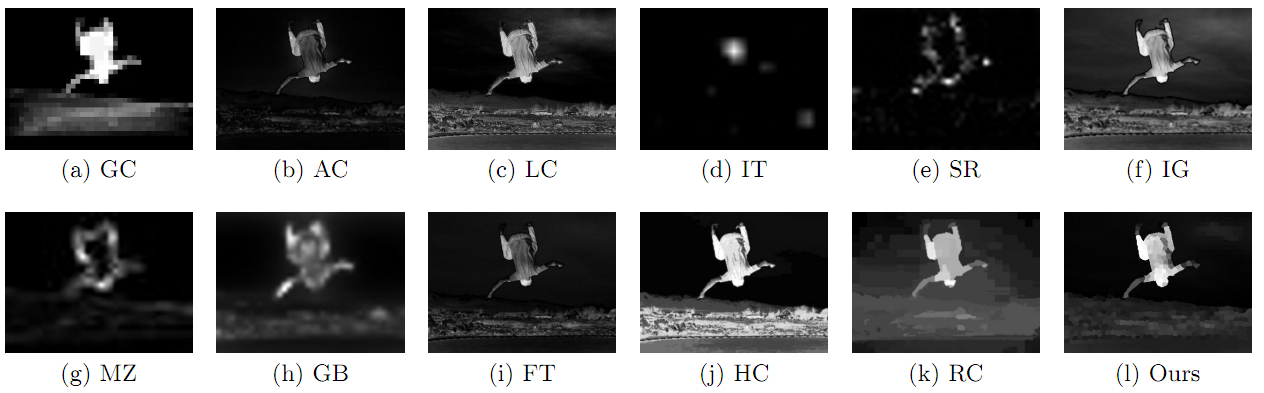
\includegraphics[width=\textwidth]{mcs-example.jpg}
\caption{与其余10种方法的对比示例}\label{fig:mcs_comp}
\end{figure}
而这些基于底层特征而计算得到的显著图在许多方面都有非常明显的、可以改进的方面。如图\ref{fig:mcs_comp}所示,基于局部对比度的方法,如MZ\cite{ma2003contrast},倾向于高亮物体的边缘,而基于全局对比度的方法如HC\cite{cheng2011global},则会将草地也一起高亮(因为草地与前景颜色相近,相对于天空同样具有较大的对比度)。而实际上,这些方法都可以在某种程度上进行修正。首先,如果一个区域被显著的区域所包围,那么这个区域也通常是显著的,这可以解决基于局部对比度的方法的缺陷;其次,如果一个区域与图像的边框相连接,那么这个区域通常不是显著的,这可以一定程度上解决基于全局对比度的方法的缺陷。所以,如果能加入这种空间上的约束,那么检测的准确率和召回率可以大大得以提高。

然而,这三种空间特征都是二值特征,很难直接将其应用到显著图中,为此我们考虑使用蒙特卡洛采样,将显著值的度量分解为多次采样-标记的过程。

\subsection{解决方法概要}
\begin{figure}
\centering
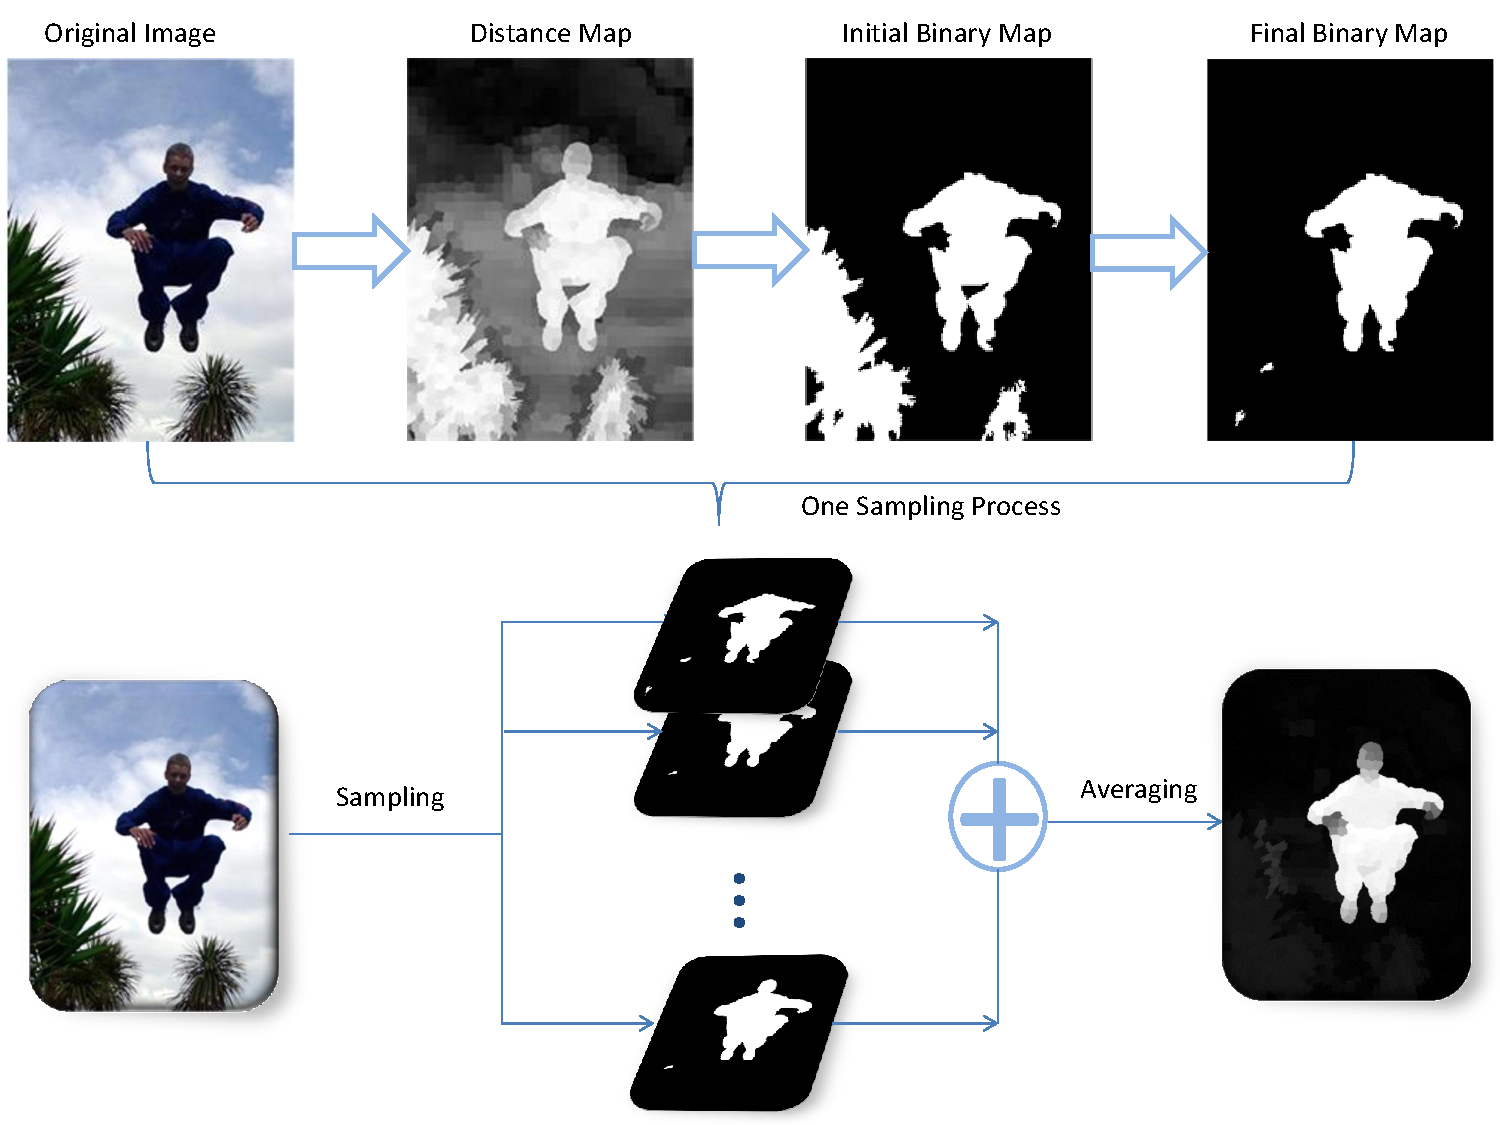
\includegraphics[width=\textwidth]{MCS.pdf}
\caption{系统框架图}\label{fig:mcs}
\end{figure}

我们为了将三种空间特征利用起来,使用了蒙特卡洛采样,将显著值的度量分解为多次采样,标记的过程,主要步骤如下:
\begin{enumerate}
\item 采样。对整幅图像中的像素点,以一定概率分布进行采样。
\item 对采样进行处理。对采样得到的像素点,计算整幅图像的Distance Map,继而利用紧致性和连通性计算Binary Map,最后利用包围性计算Final Binary Map。
\item 对多次采样得到的Binary Map进行加权平均,得到最终的显著图。
\end{enumerate}
整个系统的框架如图\ref{fig:mcs}所示。

\section{采样方法}
显著性区域检测和图像分割实际上非常相似,区别在于,前者仅仅将图像分割为两个部分:前景和背景。因此,在显著性区域检测中,图像的像素被自然的划分为前景和背景两类,显然,属于不同类别的像素点应该具有较大的差异,而属于同一类的像素点差异较小。根据我们的假设,为了高亮前景物体,我们应该在采样的时候尽量采样背景像素,这样得到的distance map中,前景物体则会被高亮,背景物体则会呈现灰暗。

根据心理学家的分析\cite{tatler2007central},人类的注意力倾向于图像中心区域,同时摄影师在摄影时,也倾向于将主体部分放置在靠近中心的位置。因此,靠近图像中心的像素点,有较大概率为前景,而靠近图像边缘的像素点,则有较大概率为背景像素。因此,为了以较大概率采样得到背景像素点,我们将采样的概率分布设定如下:
\begin{equation}
p(I_i) = \frac{1}{Z}(1-exp\{-\lambda(x_i-x_c)^2\})
\end{equation}
这里,$I_i$代表图像中的第$i$个像素点,$p(I_i)$表示该像素点被采样到的概率,$x_i$是该点的坐标,$x_c$是图像中心的坐标,$Z$是归一化因子。

\section{生成显著图}
\subsection{生成距离图}
一旦我们采样得到一个像素点,我们就可以通过以下公式计算整幅图中其他像素点与这个像素的差异:
\begin{equation}
D(I_i) = ||f_i - f_s|| \label{eq:dis}
\end{equation}
这里$f_i$是第$i$个像素点的特征向量,$f_s$是采样点的特征向量。$||*||$为欧氏距离算子。在我们的工作中,我们选取Lab颜色空间的颜色向量作为特征向量。然后我们通过归一化,将其归一化到0和1之间,得到distance map。

由于得到的距离中,存在一些异常高的值,因而使用通常的MIN-MAX归一化会使某些单一的像素高亮,而整幅图像比较暗淡。因此,我们采用下面的方法进行归一化:
\begin{equation}
D = 
\begin{cases}
1& d \geq a\\
(d-u)/(a-u) & u<d<a\\
0& d \leq u
\end{cases}
\end{equation}
这里d是由公式\ref{eq:dis}计算得到的距离,$a$和$u$都是根据自适应的图像参数。$a$被设置为使至少有5\%的像素值大于a,u被设置为至少有5\%的像素值小于u。

\subsection{生成初始二值标记图}
我们通过阈值化distance map获得二值标记图,如下所示:
\begin{equation}
B(I)= \textbf{THRESH}(D(I), \theta)
\end{equation}
然而,如何选取一个合适的阈值是非常困难的事情。正如之前所说的,我们的方法结合了三种空间特征,这里,我们使用紧致性和连通性来确定一个合适的阈值。

根据我们的观察,一个二值图标记的显著区域通常比较集中,且形成一个连通的区域。我们将二值图在空间上分布的方差作为考量紧致性的指标:
\begin{equation}
BinMap_{Var} = Var_X + Var_Y
\end{equation}
其中
\begin{equation}
Var_X = \frac{1}{N} \sum_{i=1}^N |x_i-x_c|
\end{equation}
\begin{equation}
Var_Y = \frac{1}{N} \sum_{i=1}^N |y_i-y_c|
\end{equation}
$N$是被标记为显著的像素数量,$(x_i,y_i)$则是第$i$个像素的坐标,$(x_c,y_c)$是所有被标记为显著的像素的中心。

对于连通性,我们考虑显著像素的8邻域内显著像素的数量,数量越多,说明连通性越好:
\begin{equation}
BinMap_{Con} = \frac{1}{N}\sum_{p\in I_{Sal}}\sum_{(x,y)\in N_p}\emph{1}(p_{xy})
\end{equation}
其中,$I_{Sal}$为二值图中显著像素的集合,N是该集合的大小,$N_p$是像素$p$的8邻域的坐标,$1(p_{xy})$则是判定函数,用于判定在$(x,y)$的像素点$p_{xy}$是否为显著像素。

显然,高连通性,空间分布越集中的二值图更好,因此,我们将阈值通过以下公式确定:
\begin{equation}
Criterion = \frac{BinMap_{Con}}{BinMap_{Var}}
\end{equation}
在我们的实现中,我们选取了均匀选取了9个不同的阈值,并获得了9副不同的显著图,然后,我们通过上面的式子,$Criterion$最高的显著图将被选取为初始的二值标记图。

\subsection{生成最终的二值标记图}
通过包络性,我们可以进一步优化二值标记图。根据Gestalt原理\cite{beardslee1958readings},一个有着封闭轮廓的区域更加易于被人眼理解为一个整体的实物,因而抓住人眼的注意力。

\begin{figure}
\centering
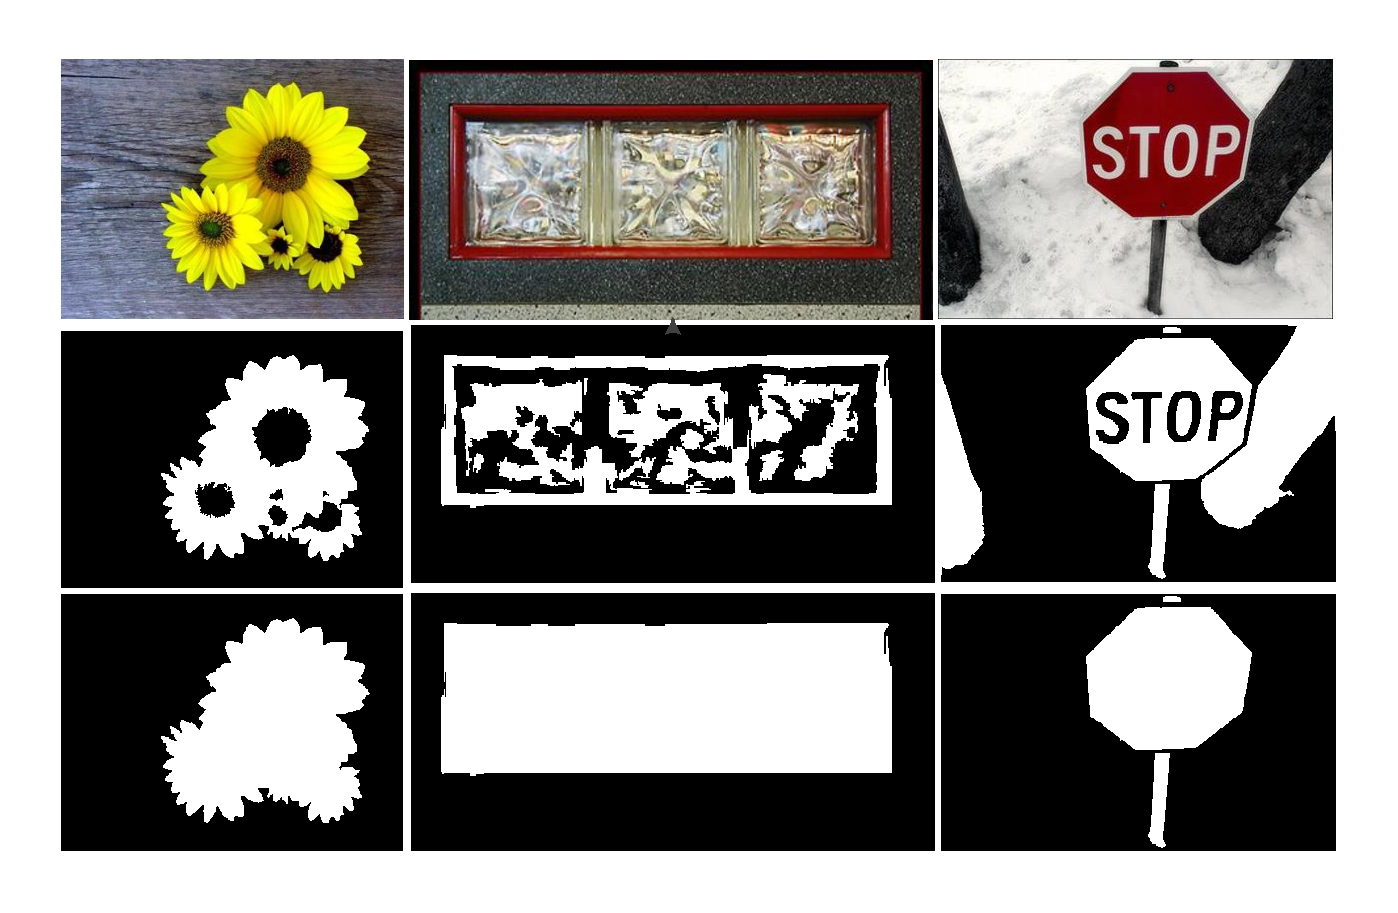
\includegraphics[width=\textwidth]{constraint.pdf}
\caption{包络性的作用} \label{fig:constraint}
\end{figure}

我们将包络性定义为二值图中有着封闭轮廓的区域,在这个定义下,任何与图像边缘连通的区域将被标记为0(背景区域),其余的区域则被标记为1(前景区域)。我们可以通过泛洪法填充,在$O(n)$的时间内标记出所有的像素点。

在图\ref{fig:constraint}中,上面一行为原图像,中间一行为初始二值标记图,下面一行为通过包络性优化过的最终的二值标记图,可以看到,通过这一简单的优化,可以大大提高二值标记图的质量。

\subsection{生成显著图}
在每一次采样后,我们都会得到一幅二值标记图,其中1标记为这次采样中,认为该像素为显著区域。根据蒙特卡洛采样原理,一个像素为显著值(即它被标记为显著的概率)最终可以用整个采样过程中,其被标记为1的频率替代(当采样次数足够多时)。因此,我们最后简单的将所有得到的二值图进行加和平均,即:
\begin{equation}
Sal(I) = \frac{1}{T}\sum_{i=1}^{N}BinMap_i(I)
\end{equation}
这里$T$是采样的次数,$BinMap_i(I)$是在第$i$次采样过程中得到的二值图。在我们的实现中,我们设置$T=400$。

\section{效率问题}
倘若直接在原图像上去进行上面的计算,由于像素数量之多,会导致时间复杂度将十分巨大。为了加速上述采样过程,我们使用了一下两个工具用于加速:
\begin{enumerate}
\item SLIC超像素分割算法\cite{achanta2010slic}。我们将整幅图像分割为超像素,之后所有的计算都以超像素为单元进行计算,这样可以使得像素数量下降许多。
\item 并行采样。由于每一次采样过程都是相互独立的,因此可以非常方便的将所有采样过程并行计算。由于我们的测试环境为4核cpu,我们将采样的线程数设置为4。
\end{enumerate}

\section{实验结果}
我们分别在ASD\cite{achanta2009frequency}和ECSSD\cite{yan2013hierarchical}这两个公开数据集上进行了我们的实验。同时与11中国际经典算法进行了对比,包括IT98\cite{itti1998model}, MZ03\cite{ma2003contrast}, LC06\cite{zhai2006visual}, GB06\cite{harel2006graph}, SR07\cite{hou2007saliency},  AC08\cite{achanta2008salient}, FT09\cite{achanta2009frequency},  IG09\cite{achanta2009frequency}, HC11\cite{cheng2011global}, RC11\cite{cheng2011global}, and GS12\cite{wei2012geodesic}。

\subsection{在ASD数据集上的结果}
\begin{figure}
\centering
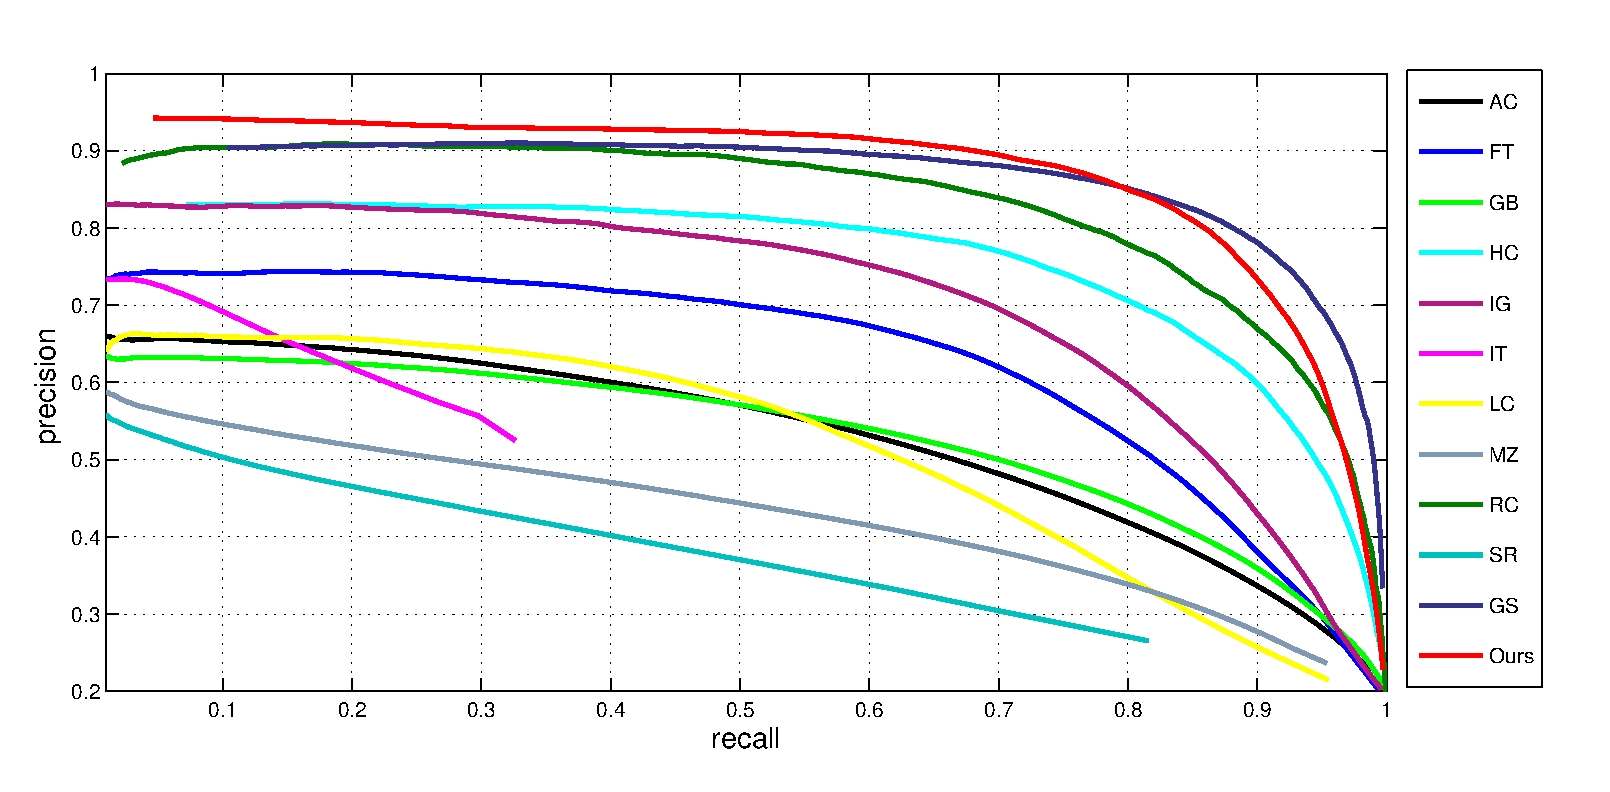
\includegraphics[width=\textwidth]{mcs_pr_curve.eps}
\caption{ASD数据集上与其他10种方法的对比:准确率-召回率曲线}
\label{fig:results2_pr}
\end{figure}
\begin{figure}
\centering
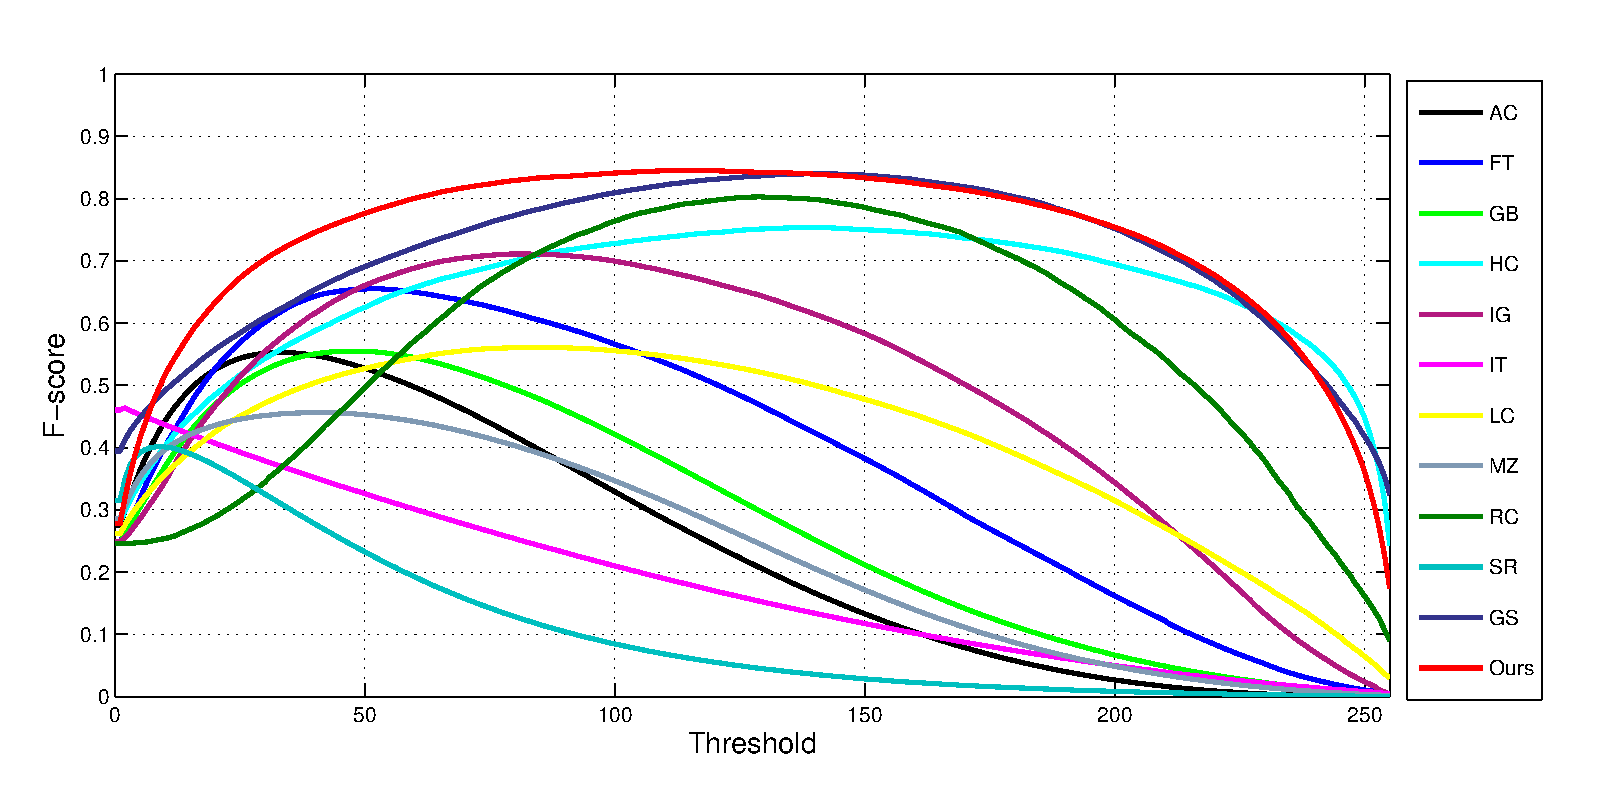
\includegraphics[width=\textwidth]{mcs_f.eps}
\caption{ASD数据集上与其他10种方法的对比:F-score曲线}
\label{fig:results2_fscore}
\end{figure}
\begin{figure}
\centering
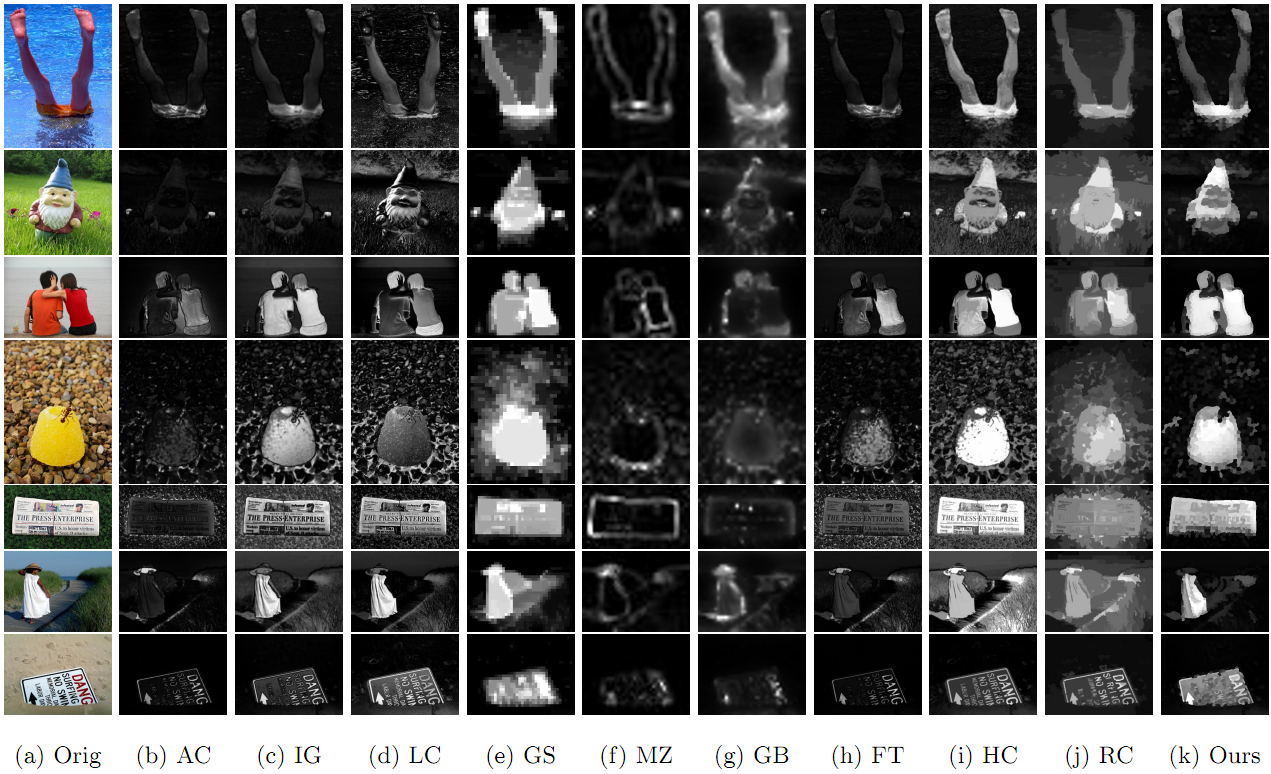
\includegraphics[width=\textwidth]{mcs_vcomp.jpg}
\caption{ASD数据集上与其他10种方法的主观视觉对比}\label{fig:vresult2}
\end{figure}
可以看到,我们的方法在ASD数据集上有很好的表现,与GS方法有非常接近的性能。尽管GS方法在召回率大于0.8的时候有更高的准确率,我们的方法在召回率低于0.8时,拥有更高的性能。同时,从F-score中可以看到,我们的方法在很大的阈值范围内均有非常良好的表现,这说明了我们的方法对阈值的选取不敏感,有一定的鲁棒性。

\subsection{在ECSSD数据集上的结果}
\begin{figure}
\centering
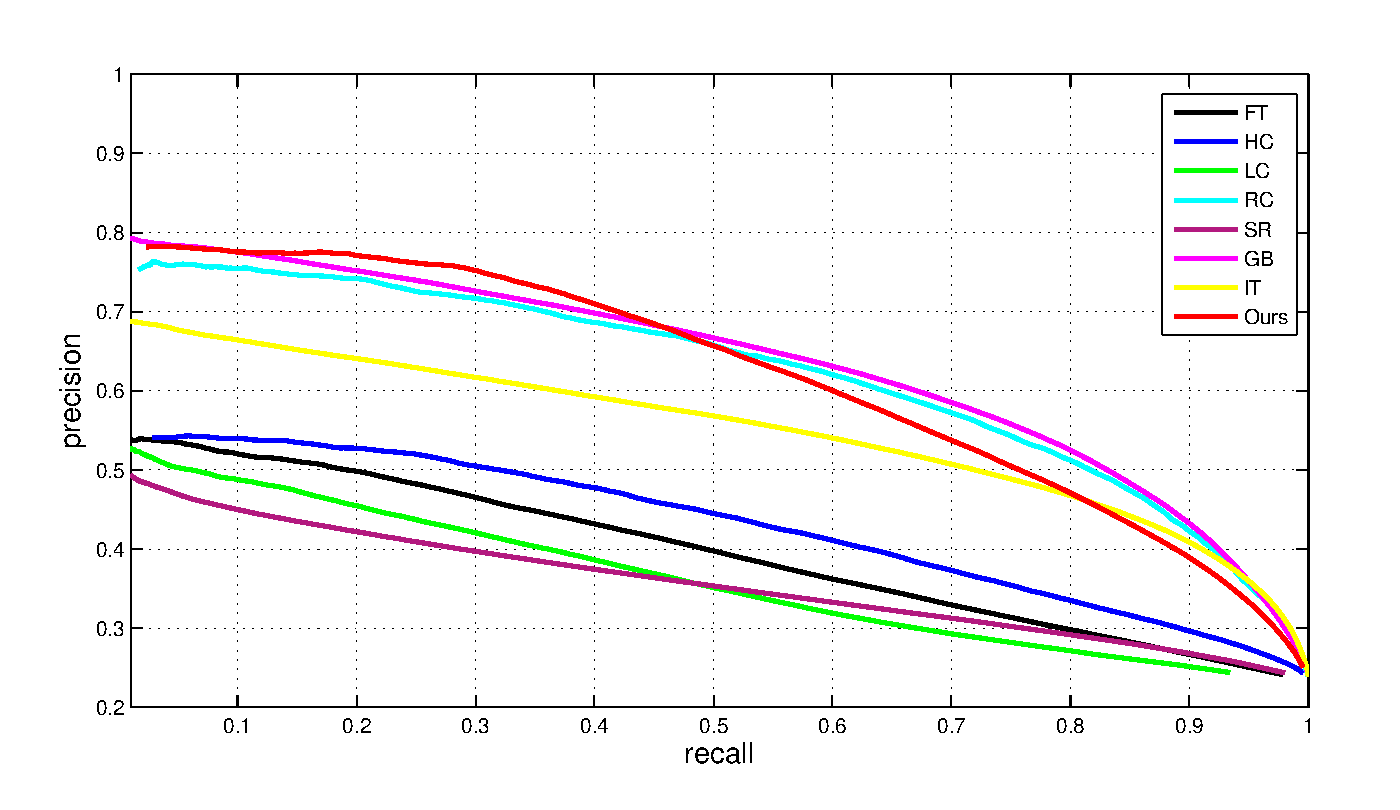
\includegraphics[width=\textwidth]{pr_curve_ecssd.eps}
\caption{ECSSD数据集上与其他10种方法的对比:准确率-召回率曲线}
\label{fig:results2_pr_ecssd}
\end{figure}
\begin{figure}
\centering
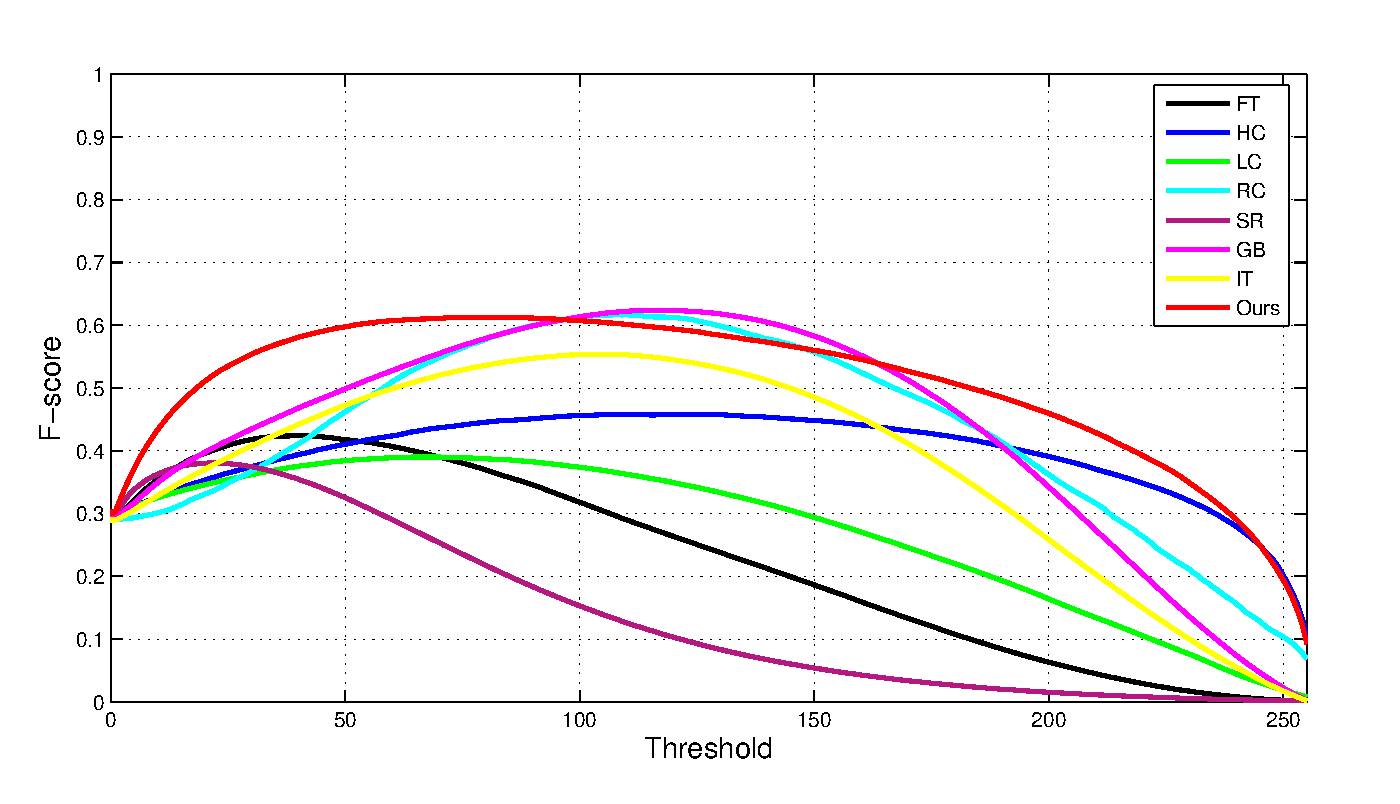
\includegraphics[width=\textwidth]{f_ecssd.eps}
\caption{ECSSD数据集上与其他10种方法的对比:F-score曲线}
\label{fig:results2_fscore_ecssd}
\end{figure}
\begin{figure}
\centering
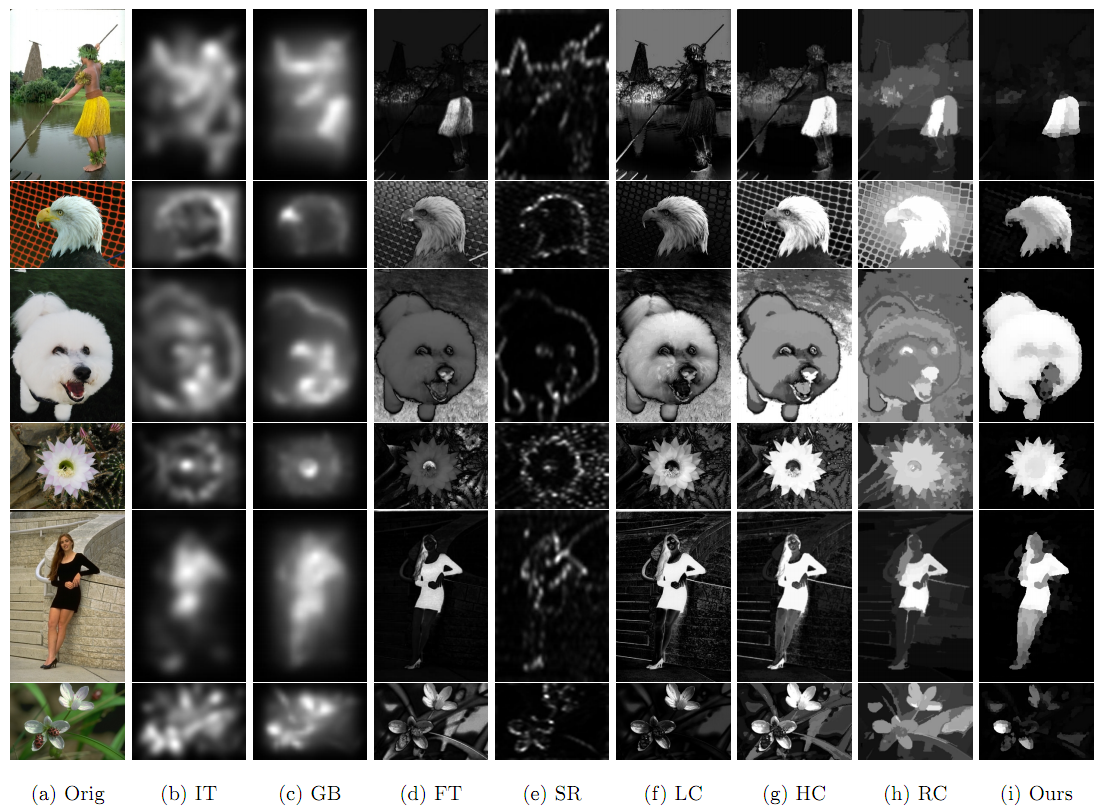
\includegraphics[width=\textwidth]{vresult_ecssd.png}
\caption{ECSSD数据集上与其他10种方法的主观视觉对比}\label{fig:vresult2_ecssd}
\end{figure}
ECSSD是一个更加有挑战性的数据集,包含了1000幅背景结构复杂的图片。由于找不到AC,IG,GS方法在这个数据集上的结果,作者也没有公开源码,因此我们仅仅比较剩余的方法。

从图\ref{fig:results2_pr_ecssd}和图\ref{fig:results2_fscore_ecssd}可以看到,我们的方法在这个数据集上依然保持竞争力。显然,由于数据集的背景结构更加,所有的方法在这个数据集上的表现都有所下降。在图\ref{fig:vresult2_ecssd}中,我们列出了两个我们的方法表现较差的图像(第一行和最后一行)。在这样的图像中,前景图像要么对比度很低(比如第一行中人的身体),要么空间先验不起作用(比如最后一行中,花朵与图像的边缘连接在了一起)。在这类图像中,底层特征已经失去了判别力,无法体现人的视觉显著性。


